\begin{frame}{Technique Comparison - List}

\begin{center}
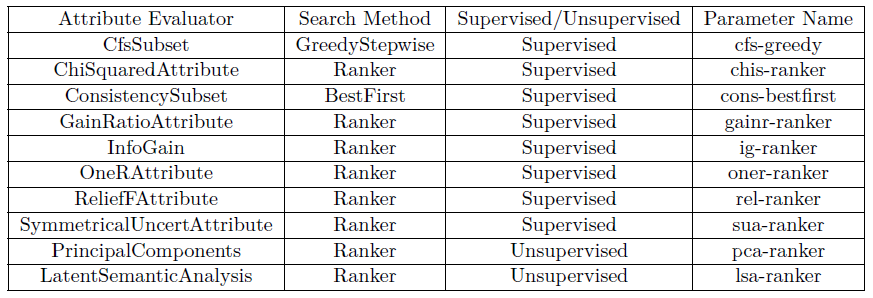
\includegraphics[scale=0.5]{fig/techniques-list.png}
\end{center}

\end{frame}

\begin{frame}{Technique Comparison - Analyze Mutual Attributes}

\bi
  \mi Unsupervised methods not interpretable
  \mi Comparison between each pair of supervised methods
  \mi Creating distance matrix
  \mi Clustering more similar ones
\ei

\end{frame}

\begin{frame}{Technique Comparison - Distance Matrix}

\begin{center}
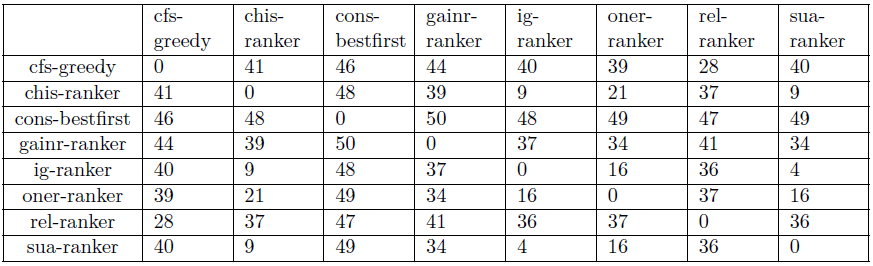
\includegraphics[scale=0.5]{fig/techniques-dismat.png}
\end{center}

\end{frame}


\begin{frame}{Technique Comparison - Clustering}

\begin{center}
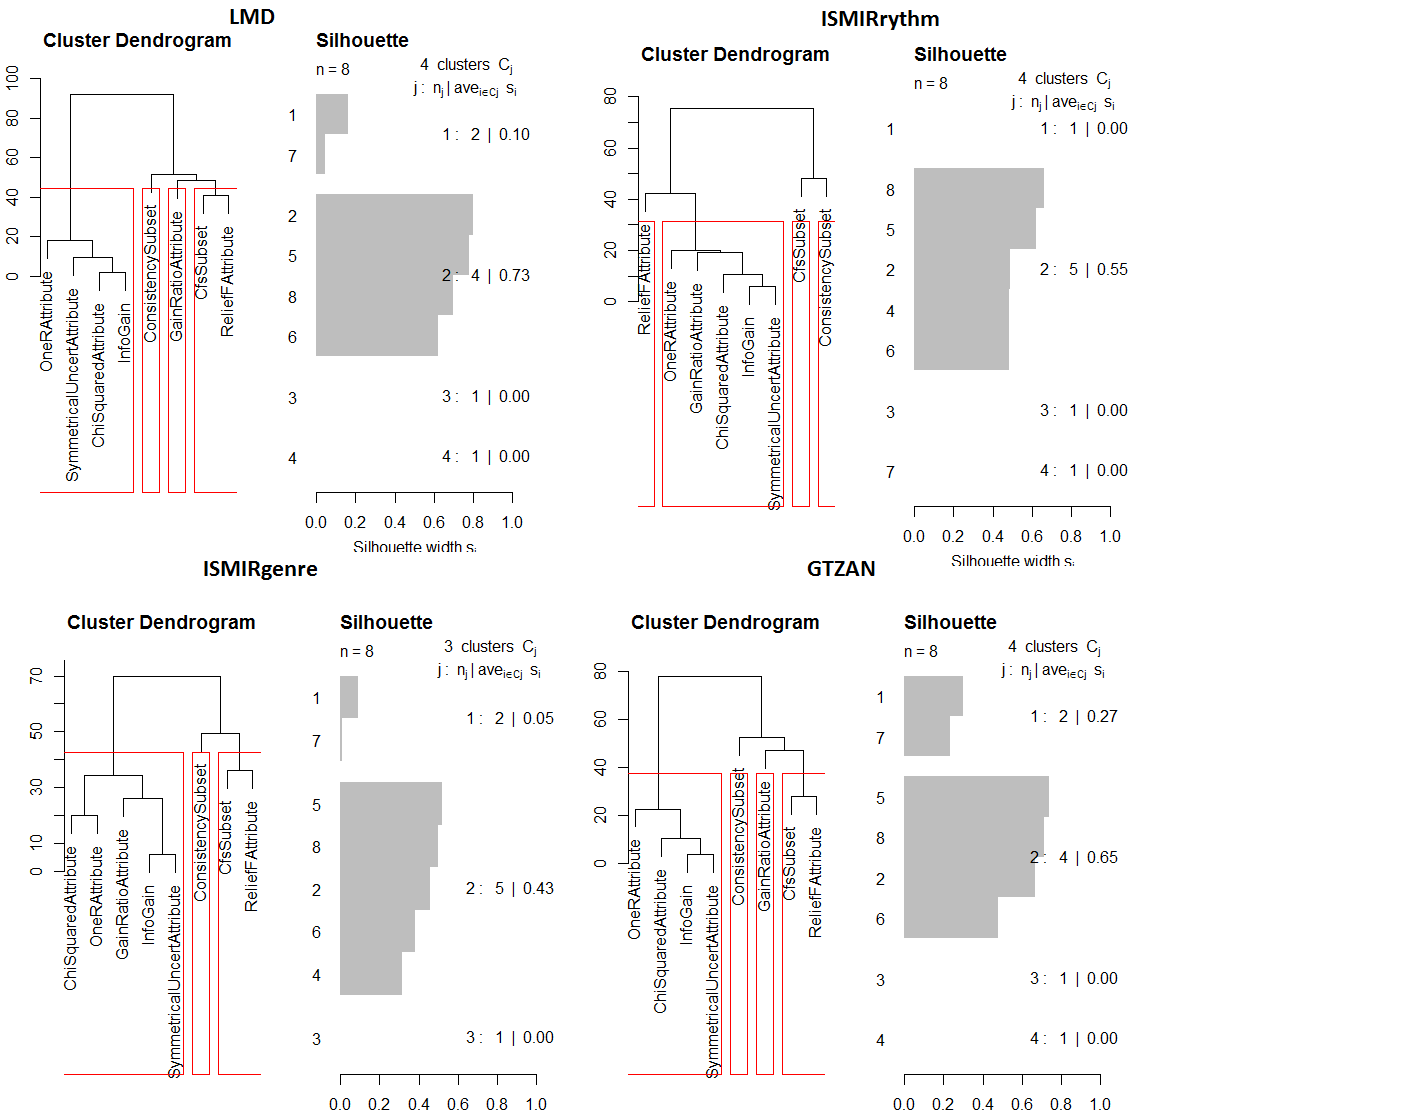
\includegraphics[scale=0.25]{fig/techniques-diagram.png}
\end{center}

\end{frame}

\begin{frame}{Technique Comparison - Conclusion}

\bi
  \mi ChiSquaredAttribute and InfoGain tend to have very similar results.
  \mi Besides ChiSquaredAttribute and InfoGain, SymmetricalUncertAttribute is the most similar one to them.
  \mi ConsistencySubset has always the most different results in comparison to the others.
  \mi CfsSubset and ReliefFAttribute seems to be related in some cases
\ei

\end{frame}

